\documentclass{beamer}

\usepackage{amsmath, amssymb}
\usepackage{graphicx}
\usepackage{url}
\usepackage{xspace}
\usepackage{pifont}
\usepackage{minted}
\usepackage{verbatim}
\usepackage{wasysym}
\usepackage{manfnt}
\usepackage{dictsym}
\usepackage[numberedbib]{apacite}
\usepackage{bm}

\DeclareMathOperator{\Tr}{Tr}
\DeclareMathOperator*{\argmin}{arg\,min}

\usetheme{AnnArbor}
\usefonttheme[onlymath]{serif}

\title[Intro DNNs]{\textbf{Practical Deep Neural Networks} \\
\textbf{\normalsize GPU computing perspective}\\
\normalsize Feedforwad Neural Networks}
\author{Yuhuang Hu \and Chu Kiong Loo}
\institute[UM]{Advanced Robotic Lab\\
Department of Artificial Intelligence\\
Faculty of Computer Science \& IT\\
University of Malaya}

\date{}

\begin{document}

\frame{\titlepage}

\begin{frame}
  \frametitle{Outline}

  \tableofcontents
\end{frame}

\AtBeginSection[]
  {
     \begin{frame}
     \frametitle{Outline}
     \tableofcontents[currentsection]
     \end{frame}
  }

\section{Introduction}

\begin{frame}
  \frametitle{Assumed prerequisites}

  \begin{itemize}
    \item[\ding{80}] Numerical Computation [DL book chapter 4]
    \item[\ding{80}] Machine Learning Basics [DL book chapter 5]
  \end{itemize}
\end{frame}

\begin{frame}
  \frametitle{Suggest Readings}

  \begin{itemize}
    \item[\ding{45}] UFLDL Tutorial: \href{http://ufldl.stanford.edu/tutorial/supervised/MultiLayerNeuralNetworks/}{Multi-Layer Neural Network}
    \item[\ding{45}] Deep Learning book: \href{http://www.iro.umontreal.ca/~bengioy/dlbook/mlp.html}{Feedforward Deep Networks}
    \item[\ding{45}] CS231n: Neural Networks \href{http://cs231n.github.io/neural-networks-1/}{Part 1}, \href{http://cs231n.github.io/neural-networks-2/}{Part 2}, \href{http://cs231n.github.io/neural-networks-3/}{Part 3}.
    \item[\ding{45}] Pattern Recognition and Machine Learning: Chapter 5
  \end{itemize}
\end{frame}

\section{Multi Layer Perceptron}

\begin{frame}
  \frametitle{Neuron}

  \begin{figure}
    \centering
    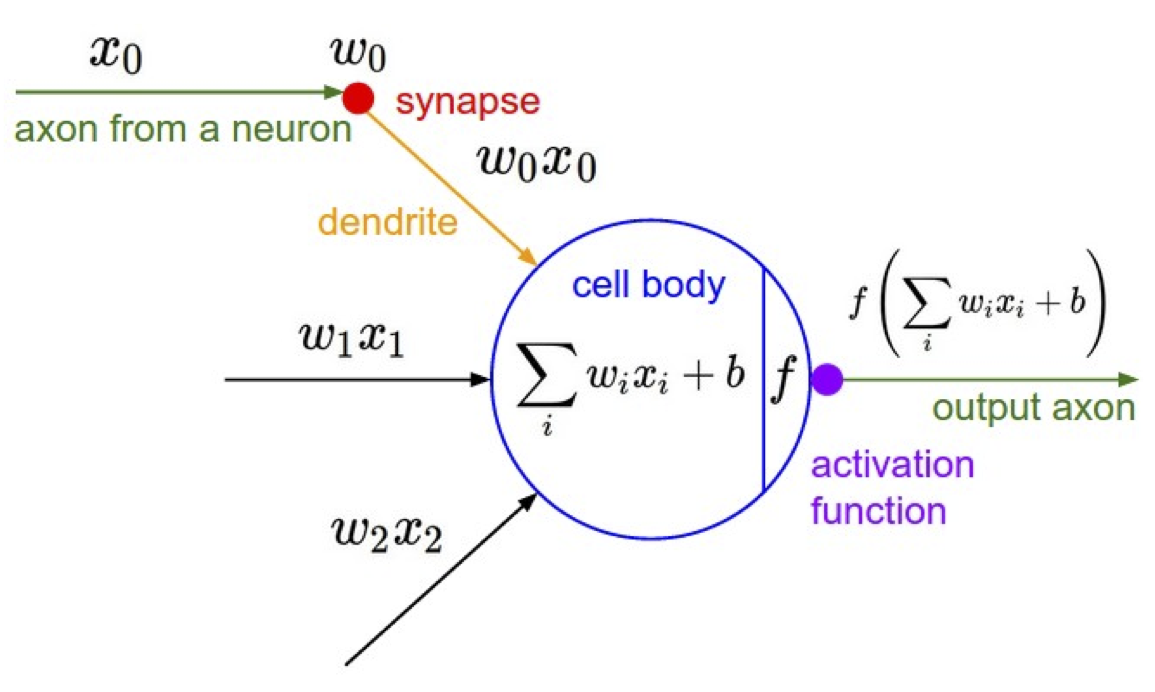
\includegraphics[width=0.7\textwidth]{neuron.png}
  \end{figure}
\end{frame}

\begin{frame}
  \frametitle{Activation function: Sigmoid}

  \begin{minipage}{0.48\textwidth}
    \begin{figure}
      \centering
      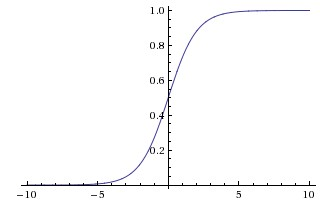
\includegraphics[width=0.8\textwidth]{sigmoid.jpeg}
      \caption{Sigmoid}
    \end{figure}
  \end{minipage}
  \begin{minipage}{0.48\textwidth}
    \begin{itemize}
      \item $f(x)=\frac{1}{1+\exp(-x)}$
      \item[\ding{51}] Rescale numbers to $[0,1]$
      \item[\ding{51}] Historically, it's very popular since it's nice to interpret ``firing rate''.
      \item[\ding{55}] Saturated neurons ``kill'' the gradients
      \item[\ding{55}] Sigmoid outputs are not zero-centered
    \end{itemize}
  \end{minipage}
\end{frame}

\begin{frame}
  \frametitle{Activation function: $\tanh$}

  \begin{minipage}{0.48\textwidth}
    \begin{figure}
      \centering
      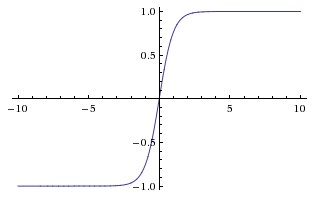
\includegraphics[width=0.8\textwidth]{tanh.jpeg}
      \caption{$\tanh$}
    \end{figure}
  \end{minipage}
  \begin{minipage}{0.48\textwidth}
    \begin{itemize}
      \item $f(x)=\frac{\exp(x)-\exp(-x)}{\exp(x)+\exp(-x)}$
      \item[\ding{51}] Rescale numbers to $[-1,1]$
      \item[\ding{51}] Output is zero-centered
      \item[\ding{55}] Still ``kill'' gradients saturated
    \end{itemize}
  \end{minipage}
\end{frame}

\begin{frame}
  \frametitle{Activation function: ReLU}
  \begin{minipage}{0.48\textwidth}
    \begin{figure}
      \centering
      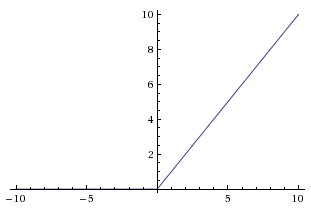
\includegraphics[width=0.8\textwidth]{relu.jpeg}
      \caption{ReLU}
    \end{figure}
  \end{minipage}
  \begin{minipage}{0.48\textwidth}
    \begin{itemize}
      \item $f(x)=\max(0,x)$
      \item[\ding{51}] Does not saturate
      \item[\ding{51}] Very computationally efficient
      \item[\ding{51}] Converge much faster than sigmoid/$\tanh$ in practice
    \end{itemize}
  \end{minipage}
\end{frame}

\begin{frame}
  \frametitle{Activation function: in practice}
  \begin{itemize}
    \item[\ding{65}] Use ReLU. Be careful with your learning rates
    \item[\ding{65}] Try out $\tanh$ but don't expect much
    \item[\ding{65}] Never use sigmoid
  \end{itemize}
\end{frame}

\begin{frame}
  \frametitle{MLP Network}
  
  \begin{figure}
    \centering
    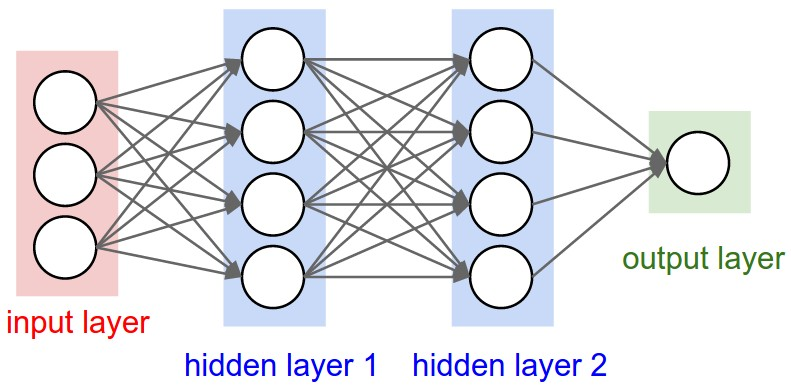
\includegraphics[width=0.7\textwidth]{neural_net.jpeg}
  \end{figure}
\end{frame}

\begin{frame}
  \frametitle{MLP Network}
  
  \begin{itemize}
    \item Layer
      \begin{equation*}
        \mathbf{h}=f_{l}(\mathbf{W}\mathbf{x}+\mathbf{b})
      \end{equation*}
    \item MLP Network Feedforward pass:

      For $l=1\ldots,n$:

      \begin{equation*}
        \mathbf{h}^{l}=f_{l}(\mathbf{W}^{l}\mathbf{h}^{l-1}+\mathbf{b}^{l})
      \end{equation*}
      where $\mathbf{h}^{0}=\mathbf{x}$.
      \begin{equation*}
        \mathbf{y}^{\text{out}}=\mathbf{h}^{n}
      \end{equation*}
  \end{itemize}
\end{frame}

\begin{frame}
  \frametitle{Cost Function}

  \begin{itemize}
    \item Let's take an example of regression:
      \begin{equation*}
        L(X, \mathbf{y}|\mathbf{W}, \mathbf{b})=\frac{1}{2N}\sum_{\mathbf{x}_{i}\in X}\left(\|y_{i}^{\text{out}}-y_{i}\|^{2}\right)
      \end{equation*}

    \item $\mathcal{L}^{2}$ regularization:

      \begin{equation*}
        L(X, \mathbf{y}|\mathbf{W}, \mathbf{b})=\frac{1}{2N}\sum_{\mathbf{x}_{i}\in X}\left(\|y_{i}^{\text{out}}-y_{i}\|^{2}\right)+\frac{\lambda}{2}\sum_{l=1}^{n}\|\mathbf{W}^{l}\|^{2}
      \end{equation*}
  \end{itemize}
  
\end{frame}

\begin{frame}
  \frametitle{Backpropagation Algorithm}
  
  \begin{itemize}
    \item Target: choose optimal parameter
      \begin{equation*}
        \mathbf{W}^{\star}, \mathbf{b}^{\star}=\argmin_{\mathbf{W}, \mathbf{b}}L(X, \mathbf{y})
      \end{equation*}
    \item Update by SGD!
      \begin{align*}
        \mathbf{W}^{*}&=\mathbf{W}-\frac{\partial}{\partial\mathbf{W}}L \\
        \mathbf{b}^{*}&=\mathbf{W}-\frac{\partial}{\partial\mathbf{b}}L
      \end{align*}
  \end{itemize}
\end{frame}

\section{Auto-Encoders}

\begin{frame}
  \frametitle{Auto-Encoder}

  \begin{itemize}
    \item[\dsheraldical] Learn hidden representation $\mathbf{h}$:
      \begin{align*}
        \mathbf{h}&=\sigma_{\text{encode}}(\mathbf{W}\mathbf{x}+\mathbf{b}) \\
        \hat{\mathbf{x}}&=\sigma_{\text{decode}}(\mathbf{W}'\mathbf{h}+\mathbf{b}')
      \end{align*}
    \item[\dsheraldical] Minimize cost (Cross-entropy cost):
      \begin{equation*}
          L(X, \hat{X})=-\frac{1}{N}\sum_{i=1}^{N}\mathbf{x}^{i}\log \hat{\mathbf{x}}^{i}+(1-\mathbf{x}^{i})\log(1-\hat{\mathbf{x}}^{i})
      \end{equation*}
  \end{itemize}
\end{frame}

\begin{frame}
  \frametitle{Denosing Auto-Encoder}
  \begin{itemize}
    \item[\dsheraldical] Idea: reconstruct input from corrupted version!
    \item[\dsheraldical] $\tilde{X}=X+\eta$, popular choices of the noise $\eta$ is binomial noise and Gaussian noise.
    \item[\dsheraldical] Learn hidden representation $\mathbf{h}$:
      \begin{align*}
        \mathbf{h}&=\sigma_{\text{encode}}(\mathbf{W}\tilde{\mathbf{x}}+\mathbf{b}) \\
        \hat{\mathbf{x}}&=\sigma_{\text{decode}}(\mathbf{W}'\mathbf{h}+\mathbf{b}')
      \end{align*}

    \item[\dsheraldical] Minimize cost (As same as previously!):
      \begin{equation*}
          L(X, \hat{X})=-\frac{1}{N}\sum_{i=1}^{N}\mathbf{x}^{i}\log \hat{\mathbf{x}}^{i}+(1-\mathbf{x}^{i})\log(1-\hat{\mathbf{x}}^{i})
      \end{equation*}
  \end{itemize}
\end{frame}

\section*{Q\&A}

\begin{frame}
  \frametitle{Q\&A}

  \begin{figure}
    \centering
    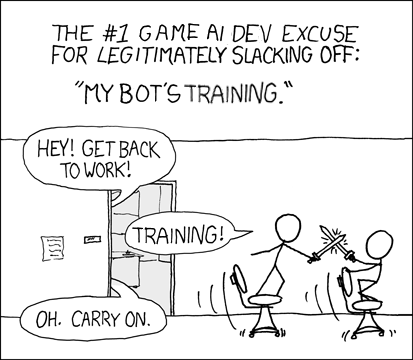
\includegraphics[width=0.65\textwidth]{training.png}
  \end{figure}
\end{frame}

\end{document}
%%% Local Variables:
%%% mode: latex
%%% TeX-master: t
%%% End:
